\section{提案手法}

先行研究により、自然言語文章生成モデルは言語モデル問題の1つとされており、式\ref{eq:generate}のように
文章$x = \mathrm{w}_1^T = (\mathrm{w}_1, \mathrm{w}_2, ..., \mathrm{w}_T)$
はある単語$\mathrm{w}_t$が生成される前の単語群$ \mathrm{w}_1^{t-1}$による条件付き確率の総積であると定義されている。

\begin{equation}
    \label{eq:generate}
    p(x) = p(\mathrm{w}_1^T) = \prod_{t=1}^{T} p(\mathrm{w}_t|\mathrm{w}_1^{t-1})
\end{equation}

提案モデルによる文章生成の流れは図\ref{fig:method}の通りである。
第\ref{subsec:generate}の通り、ベースとなったGroverモデルは記事を5要素に分けて学習が行われており、
生成及び分類学習において、各要素の始点と終点には開始及び終了トークンが付加されている。
本研究ではこれらの要素を記事本文とそれに寄せられた3件のコメントに置換することで実装する。
ベースとなったモデルに倣い、提案モデルは以下の同時分布として定義する。

\begin{equation}
    \label{eq:joint_distri}
    p(\rm{article}, \rm{comment\_1}, \rm{comment\_2}, \rm{comment\_3})
\end{equation}

コメント生成学習時は、ベースとなったGroverモデルと同様に記事とコメントのセットを2つの集団に分け、無作為に歯抜けにする。
コメントの場合は10\%、記事本文の場合は35\%の確率で歯抜けにしてから一方の集団から学習を行い、もう一方での生成におけるクロスエントロピー誤差を最小化するように訓練される\cite{NIPS2019_9106}。
提案モデルの目的は記事ではなくSNS上で記事に寄せられたユーザの反応を生成することである。

\begin{figure*}[t]
    \centering
    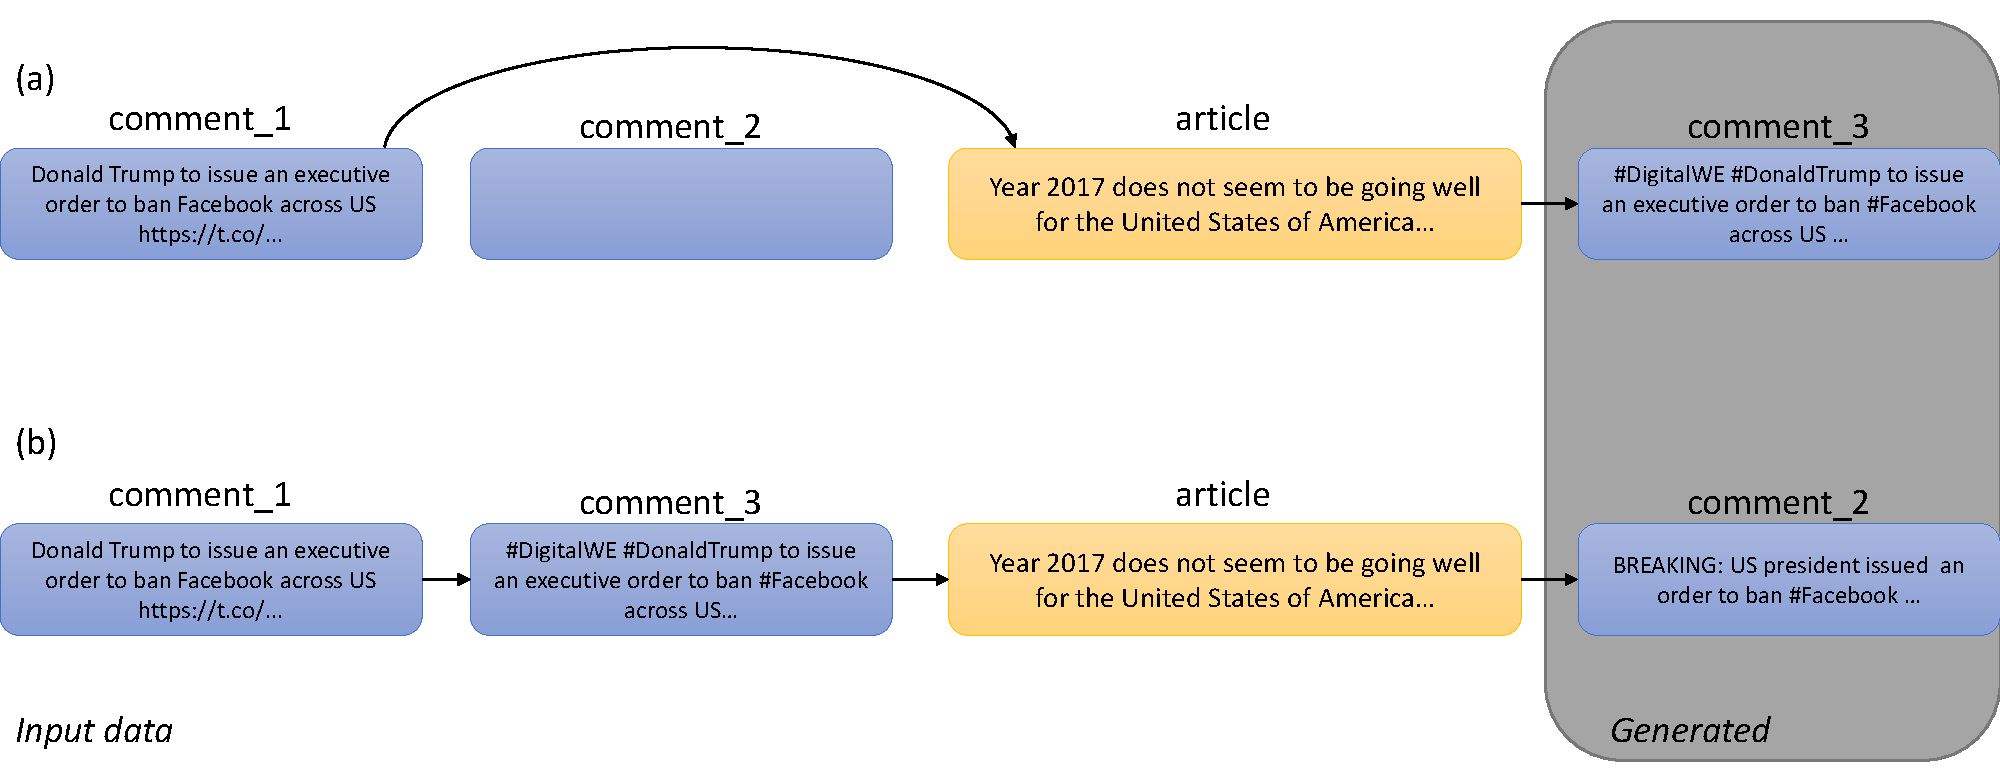
\includegraphics[width=\linewidth,pagebox=cropbox,clip]{images/fig_method.pdf}
    \caption{
        提案モデルのコメント生成例。
        (a)は記事と1件の実際に寄せられたコメントからコメントを生成している。
        (b)は(a)で生成したコメントを含めた状況で更にコメントを生成している。
    }
    \label{fig:method}
\end{figure*}

記事とコメントのセットの末尾にはセットの終端を意味するトークンである\texttt{[CLS]}を追加し、またこのトークンが真偽を分類する際に使われる。
これはGroverモデルがベースとしているGPT-2がとる手法\cite{Radford_GPT2}と同一である。
図は実際の記事とコメントのセットを真偽分類するまでの流れを示している。
まず、記事に寄せられたコメント群から実験に使用するために無作為に3件選出し、コメント生成の学習を行う。
真偽分類する際には、3件の実際に投稿されたコメントから1件削除してから生成されたコメントを追加してから真偽の分類を行う。
また、同時に生成コメントを追加しなかった状況で分類を行った際の結果との比較も行った。

\begin{figure*}[t]
    \centering
    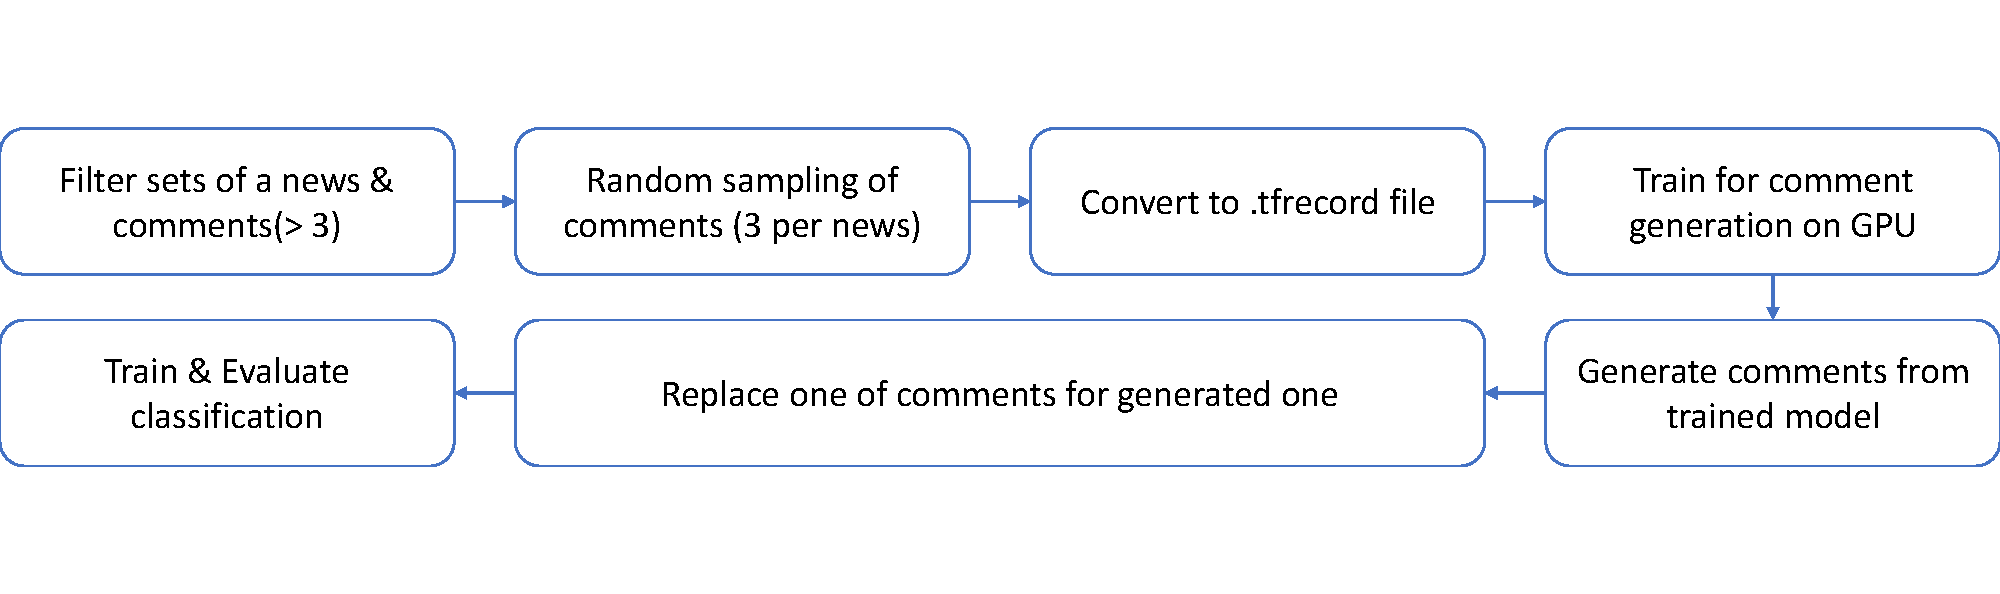
\includegraphics[width=0.8\linewidth,pagebox=cropbox,clip]{images/fig_process.pdf}
    \caption{実験の流れ}
    \label{fig:process}
\end{figure*}
